\begin{figure}[b]
\begin{minipage}{0.64\textwidth}
\resizebox{\textwidth}{!}{
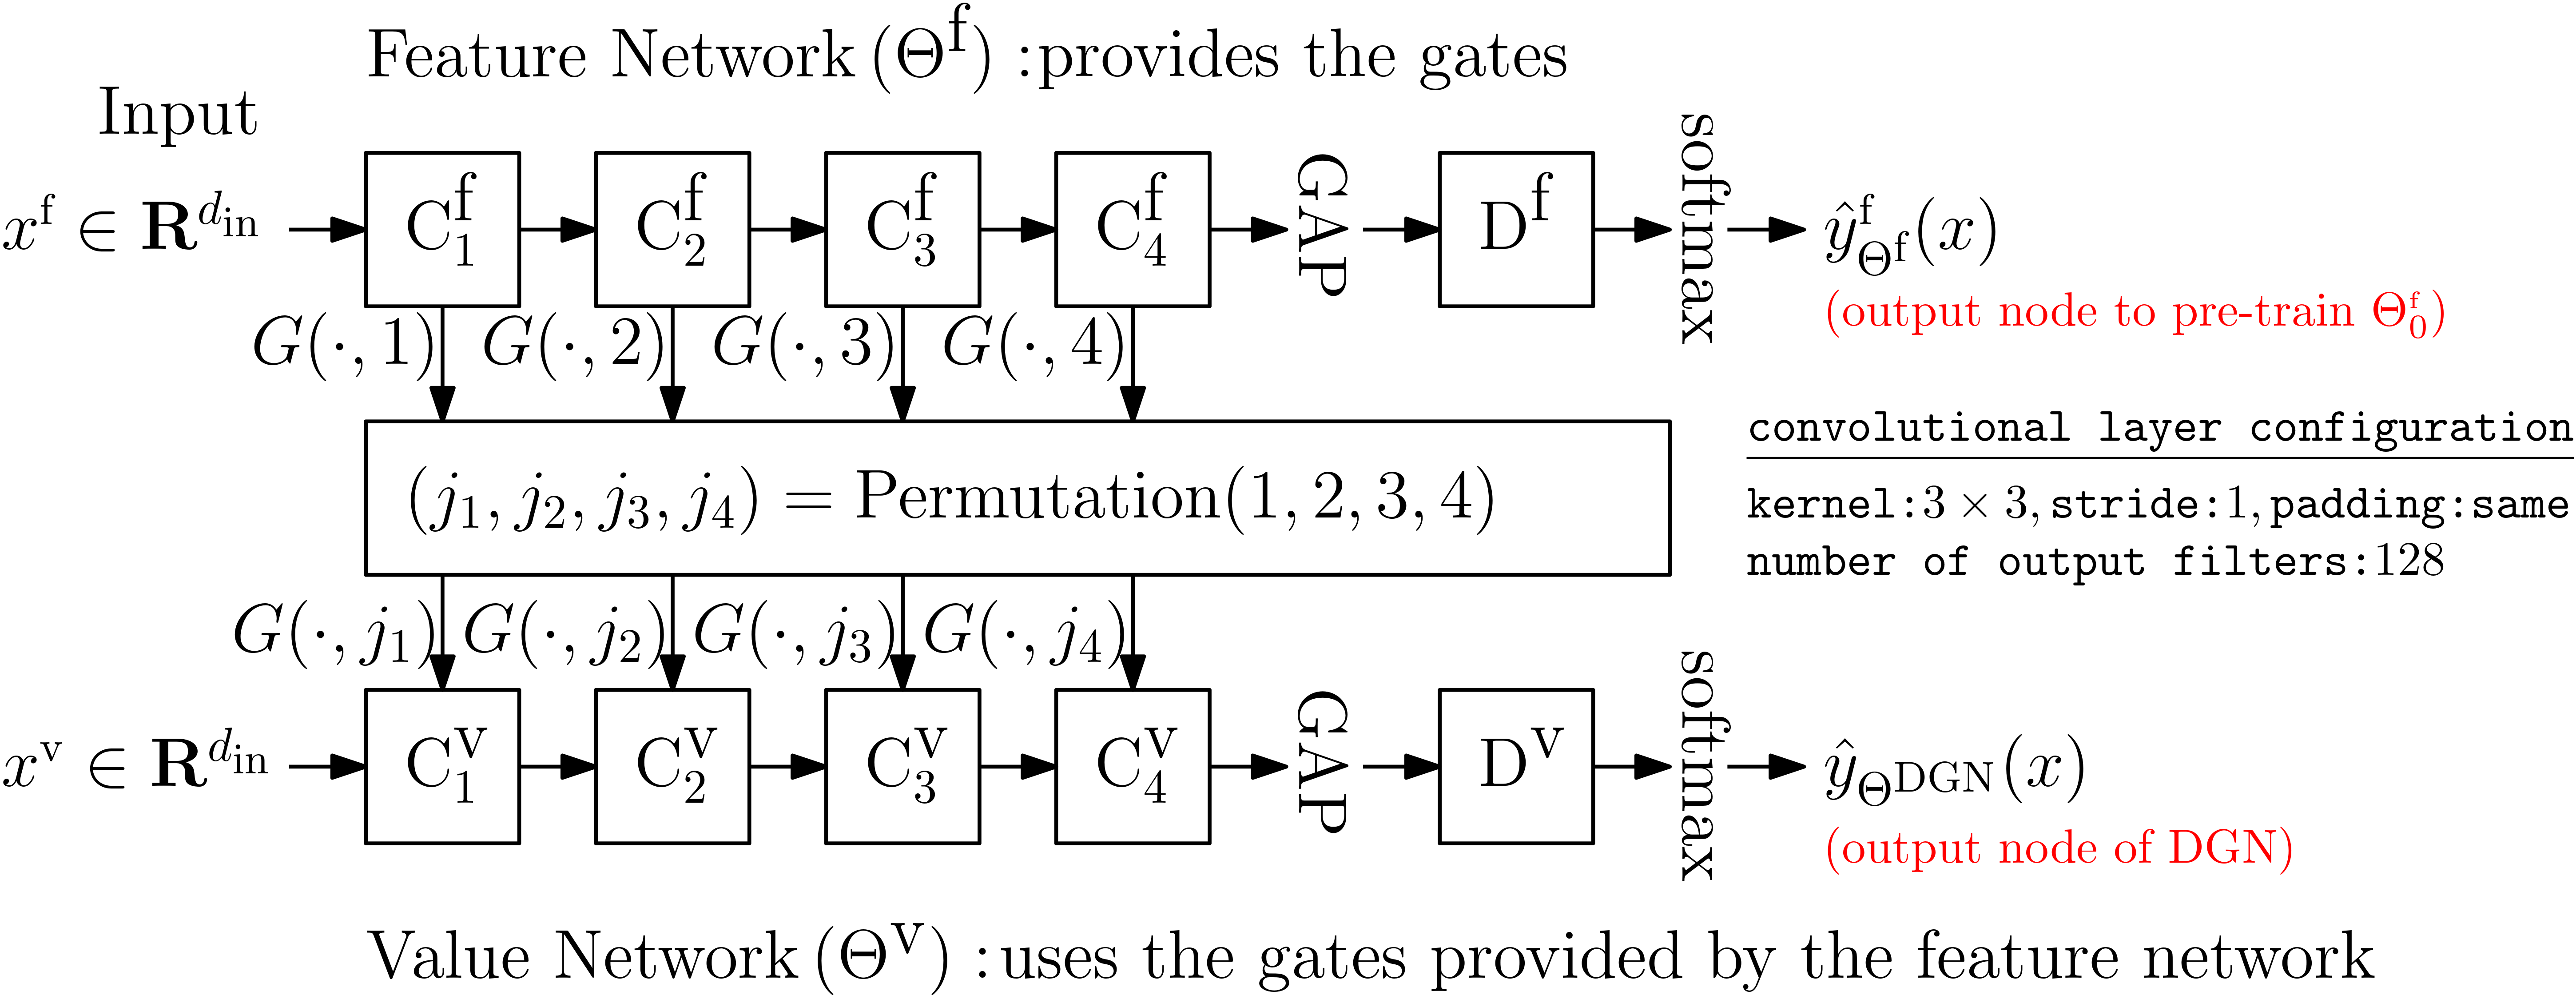
\includegraphics[scale=0.5]{figs/ablation.png}
}
\end{minipage}
\begin{minipage}{0.35\columnwidth}
\small
\resizebox{\columnwidth}{!}{
\begin{tabular}{|c|c|c|c|}\hline
&FC& CNN & ResNet\\\hline
%FR-II& $94.10\pm0.27\%$ & $67.53\pm0.73\%$\\\hline
%FR-DI& $94.06\pm0.25\%$ & $67.6\pm0.74\%$\\\hline
%DL& $98.14\pm0.07\%$ & $77.59\pm0.59\%$\\\hline
%FL& $98.62\pm0.05\%$ & $79.37\pm0.29\%$\\\hline
%ReLU& $\%$ & $\%$\\\hline
FR-II& $94.1\%$ & $67.5\%$ &$89.8\%$\\\hline
FR-DI& $94.1\%$ & $67.6\%$& $89.8\%$ \\\hline
DL& $98.1\%$ & $77.6\%$& $92.4\%$ \\\hline
FL& $98.6\%$ & $79.4\%$& $92.5\%$\\\hline
ReLU& $98.5\%$ & $80.4\%$& $93.1\%$\\\hline
\end{tabular}
}
\,In all cases, standard deviation was less than $0.5\%$. MNIST for FC, CIFAR-10 for CNN and ResNet.
\end{minipage}
\begin{comment}
\begin{minipage}{0.45\columnwidth}
\small
\resizebox{\columnwidth}{!}{
\begin{tabular}{|c|c|c|c|}\hline
& MNIST (FC)& CIFAR-10 (CNN) & CIFAR-10 (ResNet)\\\hline
%FR-II& $94.10\pm0.27\%$ & $67.53\pm0.73\%$\\\hline
%FR-DI& $94.06\pm0.25\%$ & $67.6\pm0.74\%$\\\hline
%DL& $98.14\pm0.07\%$ & $77.59\pm0.59\%$\\\hline
%FL& $98.62\pm0.05\%$ & $79.37\pm0.29\%$\\\hline
%ReLU& $\%$ & $\%$\\\hline
FR-II& $94.1\pm0.3\%$ & $67.5\pm0.7\%$ &$89.8\pm0.1\%$\\\hline
FR-DI& $94.1\pm0.3\%$ & $67.6\pm0.7\%$& $89.8\pm0.2\%$ \\\hline
DL& $98.1\pm0.1\%$ & $77.6\pm0.6\%$& $92.4\pm0.1\%$ \\\hline
FL& $98.6\pm0.1\%$ & $79.4\pm0.3\%$& $92.5\pm0.5\%$\\\hline
ReLU& $98.5\pm0.1\%$ & $80.4\pm0.3\%$& $93.1\pm0.1\%$\\\hline
\end{tabular}
}
\end{minipage}

\begin{minipage}{0.28\textwidth}
\resizebox{\columnwidth}{!}{
\begin{tabular}{|l|l|}\hline
Regimes & $\Tf$\\\hline
FR-II & R, NT\\\hline
FR-DI & R, NT, $\Tf_0=\Tv_0$\\\hline
FL & PT, NT\\\hline
DL & R, T\\\hline
\end{tabular}
}
\resizebox{\columnwidth}{!}{
\begin{tabular}{|l|l|}\hline
Mode	& Input\\\hline
Image	& $\xv=\xf=x$\\\hline
`All-Ones' & $\xf=x,\xv=\mathbf{1}$\\\hline
\end{tabular}
}
\end{minipage}
\end{comment}
\caption{\small{$\textrm{C}_i^{\text{f}},\textrm{C}_i^{\text{v}},i\in[4]$ are the convolutional layers, which are followed by \emph{global-average-pooling} (GAP) layer then by a dense layer ($\textrm{D}^{\text{f}}$/$\textrm{D}^{\text{v}}$), and a softmax layer to produce the final logits.}} %`R',  `L', `T' and `NT' stand for random, learnt, trainable and non-trainable respectively.}}
\label{fig:ablation}
\end{figure}
